\documentclass[11pt]{article}
\usepackage{amsmath,amsthm,verbatim,amssymb,amsfonts,amscd, graphicx}
\usepackage{graphicx}
\usepackage{listings}
\usepackage{float}
\usepackage{url}
\usepackage{titlesec}
\setcounter{secnumdepth}{4}


\graphicspath{{./times/}}
\topmargin0.0cm
\headheight0.0cm
\headsep0.0cm
\oddsidemargin0.0cm
\textheight23.0cm
\textwidth16.5cm
\footskip1.0cm

\titleformat{\paragraph}
{\normalfont\normalsize\bfseries}{\theparagraph}{1em}{}
\titlespacing*{\paragraph}
{0pt}{3.25ex plus 1ex minus .2ex}{1.5ex plus .2ex}


\begin{document}
\title{CS 5220\\ Project 3 - All Pairs Shortest Path}
\author{Marc Aurele Gilles (mtg79)\\ Edward Tremel (ejt64) \\ Yu Su (ys576)}
\maketitle

\section{Introduction}
In this project the goal is to profile, parallelize and tune an algorithm which computes the shortest path between all the pairs in a graph.


\section{Profiling of Original Code}
The profiling was done using amplxe. By looking at the hotspots report, we observe that most of the time (45 out of 67 seconds) is spent in the \texttt{square} function, which is to be expected as all of the computation is done in this function. A notable point, however, is that virtually all the rest of the time is spent waiting, which seems to indicate a significant load imbalance between the threads.
Looking at the time spent inside of the \texttt{square} function, we observe that a majority of the time (27 out of 45 seconds) is spent fetching memory and writing it to a float, which could indicate that there is poor cache utilization.

This profiling leads us to believe that we should try to address two problems for the OMP implementation: have better load balancing, and increase cache reuse.

Load balancing problem can be solved by tuning the communication procedure in parallelization. Before that, we try to first increase cache utilization by involving block matrix. The idea is similar to the matrix multiplication problem since they have the similar formulation. With Xeon E5-2620 v3 core with 256KB L2 cache, the block size is choosing to be 128. In the copy optimization \texttt{\_\_mm\_\_malloc} is used to allocate buffers with the byte alignment 64 bits. The reason that this byte alignment can give the best performance may be because the integer in a 64 bits core is 64 bits. In a single thread, the optimized block square function runs in 80s with n=3072, comparing with 350s of the basic loops also in a single thread. It shows that with block matrices the performance is improved significantly even without parallelization. However, directly applying \texttt{\#pragma parallel for} into the block version fails may be due to synchronization issue. Next we will modify the parallelization procedure carefully based on MPI utilizing the similar block format.


\section{MPI Implementation}
We assign each processor to a block of the the matrix instead of an entire column as the original code does.
Note that to update one entry of the matrix for one step of the outer loop we need to read the whole column and row of that entry. Therefore, if we assign each processor to a column, then each processor needs to access each other column, and thus needs to communicate with all of the other processors. By assigning each processor to a block of the matrix instead, we allow each processor to have to communicate with only the blocks that share its row and its column.

To take advantage of this blocking strategy, we create $2n_{block}$ groups and communicators, where $n_{block}=n/blocksize$. Here $n$  is the dimension of the matrix and $blocksize$ is the dimension of the blocks. That is, we have one communicator for each row of blocks, and one communicator for each column of blocks. Each thread, which owns its own block, is then added to the communicator of its row and to the communicator of its column. Therefore each thread is in two different communicators (in addition to the world communicator), but no two threads are in the same two communicators. To update its block, each processor makes one \textbf{\texttt{MPI\_Allgather}} call in its column communicator and one \textbf{ \texttt{MPI\_Allgather}} call in its row communicator, which reads all of the entries in its block column and block row, performs the update on its own block, and calls \textbf{\texttt{MPI\_Allgather}} again to share its result with the other processors.

The number of entries to be shared in this manner is $2 \cdot n \cdot blocksize$ per thread and per time step, compared to $n^2$ if each thread owned a column instead.

\section{Performance Comparison}
We measured the runtime of our MPI implementation for various numbers of processors and compared it to the original OpenMP code running with various numbers of processors.
Unfortunately, since our MPI implementation currently cannot handle non-square numbers of processors, we were only able to test it with 1, 4, and 16 processors (a maximum of 24 processors are available on the Xeon main boards).
Figure \ref{fig:mpi-omp} shows the results for numbers of processors greater than 1.
The serial versions of both programs were so slow that we plotted them on a separate graph, figure \ref{fig:serial}.

\begin{figure}[h]
	\centering
	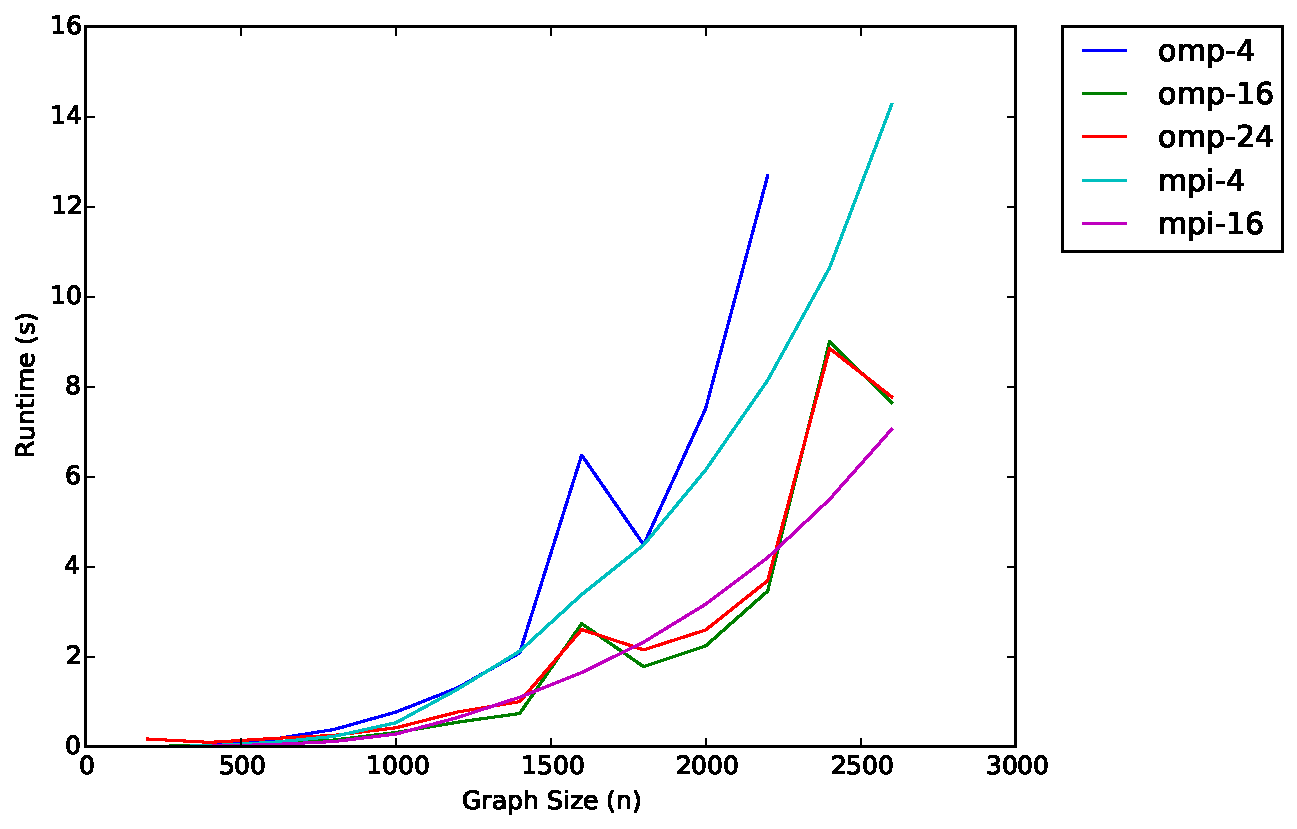
\includegraphics[width=.8\textwidth]{mpi_omp_comparison.pdf}
	\caption{Speed of the OpenMP and MPI implementations as the problem size and number of processors changes.}
	\label{fig:mpi-omp}
\end{figure}

\begin{figure}[h]
	\centering
	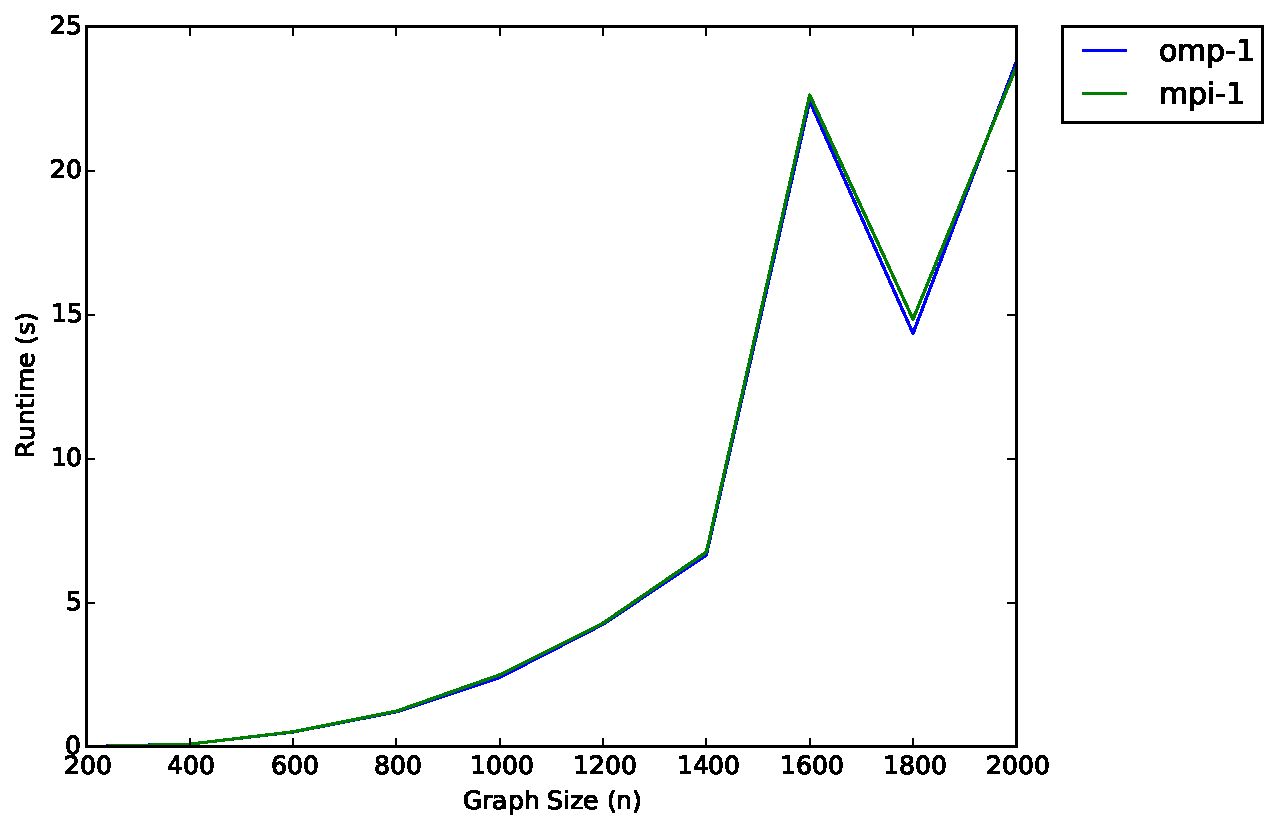
\includegraphics[width=.8\textwidth]{serial.pdf}
	\caption{Speed of the OpenMP and MPI implementations with only one processor.}
	\label{fig:serial}
\end{figure}

With a small number of processors (4), our MPI implementation runs about as well as the OpenMP code for small values of $n$, and scales much better for large values of $n$.
With 16 processors, our MPI implementation is actually a little slower than the OpenMP code at small values, and for some reason much slower for values of $n$ between 1800 and 2200.
However, for $n = 1600$ and also for large values of $n$, we again perform faster than OpenMP.


\section{Future Work}
Next we will to tune our MPI implementation as well as the OMP implementation provided to us. We will also incorporate the blocking strategy into our parallel code to increase the cache reuse.

\end{document}
